\documentclass{article}
\usepackage[T1]{fontenc}
\usepackage[polish]{babel}
\usepackage[utf8]{inputenc}
\usepackage{graphicx}
\graphicspath{{images/}}
\usepackage{blindtext}
\usepackage{hyperref}
\usepackage{placeins}
\usepackage{caption}
\usepackage{subcaption}

\title{Generacja tekstów piosenek}
\author{Maciej Krzyżanowski, Sebastian Kutny, Tomasz Lewandowski}
\date{Kwiecień 2023}

\begin{document}

\maketitle

\tableofcontents

\newpage
\section{Wstęp}
Celem projektu było stworzenie modelu generującego tekst piosenki na podstawie wybranych danych jako tekstów innych utworów. Wykorzystaliśmy 2 metody: łańcuchy Markova oraz rekurencyjne sieci neuronowe. \\ \\ Projekt zawiera narzędzie "scraper" do pozyskiwania danych ze stron: 
\begin{itemize}
    \item \url{https://www.tekstowo.pl}
    \item \url{https://www.azlyrics.com}
\end{itemize}
Implementacja została wykonana w języku Python oraz wykorzystuje biblioteki: 
\begin{itemize}
    \item pandas
    \item BeautifulSoup
    \item nltk
    \item request
    \item queue
    \item re
\end{itemize}
Dostępna jest opcja łączenia zbiorów danych do jednego pliku w celu wykorzystania ich jednocześnie. \\ \\
Przed rozpoczęciem przetwarzania danych są one oczyszczane poprzez ujednolcenie wielkości liter, usunięcie niepotrzebnych znaków interpunkcyjnych, słów zakazanych (np:. określających składowe tekstu utworu) oraz wyrażeń ze szczególnymi znakami interpunkcyjnymi jako określających zawartość tekstu.
\\ \\
Tekst jest generowany jako dowolna liczba wersów o dowolnej ilości słow.
\newpage
\section{Łańcuchy Markova}
\subsection{Wstęp}
Łańcuchy Markova to matematyczny model służący do generowania tekstu lub sekwencji innych elementów, takich jak dźwięki lub obrazy. Ideą modelu jest analiza sekwencji istniejących elementów i wykorzystanie tych informacji do przewidywania, jakie elementy powinny pojawić się następnie. \\
\\
W przypadku generowania tekstu, łańcuchy Markova są zwykle stosowane do analizy sekwencji słów w tekście źródłowym i generowania nowych sekwencji słów na podstawie tych informacji. Proces zaczyna się od wyboru deterministycznego lub losowego początkowego stanu łańcucha, a następnie generowania kolejnych stanów na podstawie informacji o pradwopodobieństwie wystąpienia po sobie stanów w analizowanym tekście w kontekście poprzednio wygenerowanych stanów. Przykładowo, jeśli w tekście źródłowym po słowie "generator" często pojawia się słowo "piosenek", to model łańcucha Markova przypisze wysokie prawdopodobieństwo wystąpienia słowa "piosenek" po słowie "generator". \\
\\
Istnieją różne sposoby implementacji modelu łańcuchów Markova, ale zwykle opierają się one na analizie pewnej liczby poprzednich elementów, zwanej "stopniem" modelu. Na przykład, w przypadku modelu pierwszego stopnia, prawdopodobieństwo wystąpienia danego elementu zależy tylko od poprzedniego elementu, w modelu drugiego stopnia, prawdopodobieństwo zależy od dwóch poprzednich elementów, a w modelu trzeciego stopnia, prawdopodobieństwo zależy od trzech poprzednich elementów itd. Stopień łańcucha nazywamy N-gramem.\\
\\
W naszym projektcie N-gram jest parametryzowany i bazuje na N uprzednio wygenerowanych słowach w wersie, losując następne słowo na podstawie prawdopodobieństwa jego wystąpienia po N sekwencji słów uprzednio wygenerowanych. Dodatkowo przy każdym wersie o nieparzystym numerze podejmowana jest próba stworzenia rymującego się wersu na podstawie ostatniej sylaby poprzedniego. Najpierw znajdowane są wszystkie rymujące się zakończenia wersu niebędące ostatnim słowem poprzedniego, a następnie - jeśli takie istnieją - losujemy jedno z nich zamiast z wszyskich pozycji. Przy nieznalezieniu rymujących się słów generacja odbywa się tak jak w zwykłym wypadku. W praktyce szansa na stworzenie rymu jest mała i powinna rosnąć z ilością danych przetwarzanych przez model.\\
\\
Model łańcuchów Markova nie jest idealny i może generować sekwencje, które nie są sensowne lub poprawne gramatycznie. Dopiero przy wglądzie modeli w setki stanów wstecz oraz przy bardzo dużej ilości danych można wygenerować tekst podobny do pisanego przez człowieka. \\
\\
\begin{figure}[h]
    \centering
    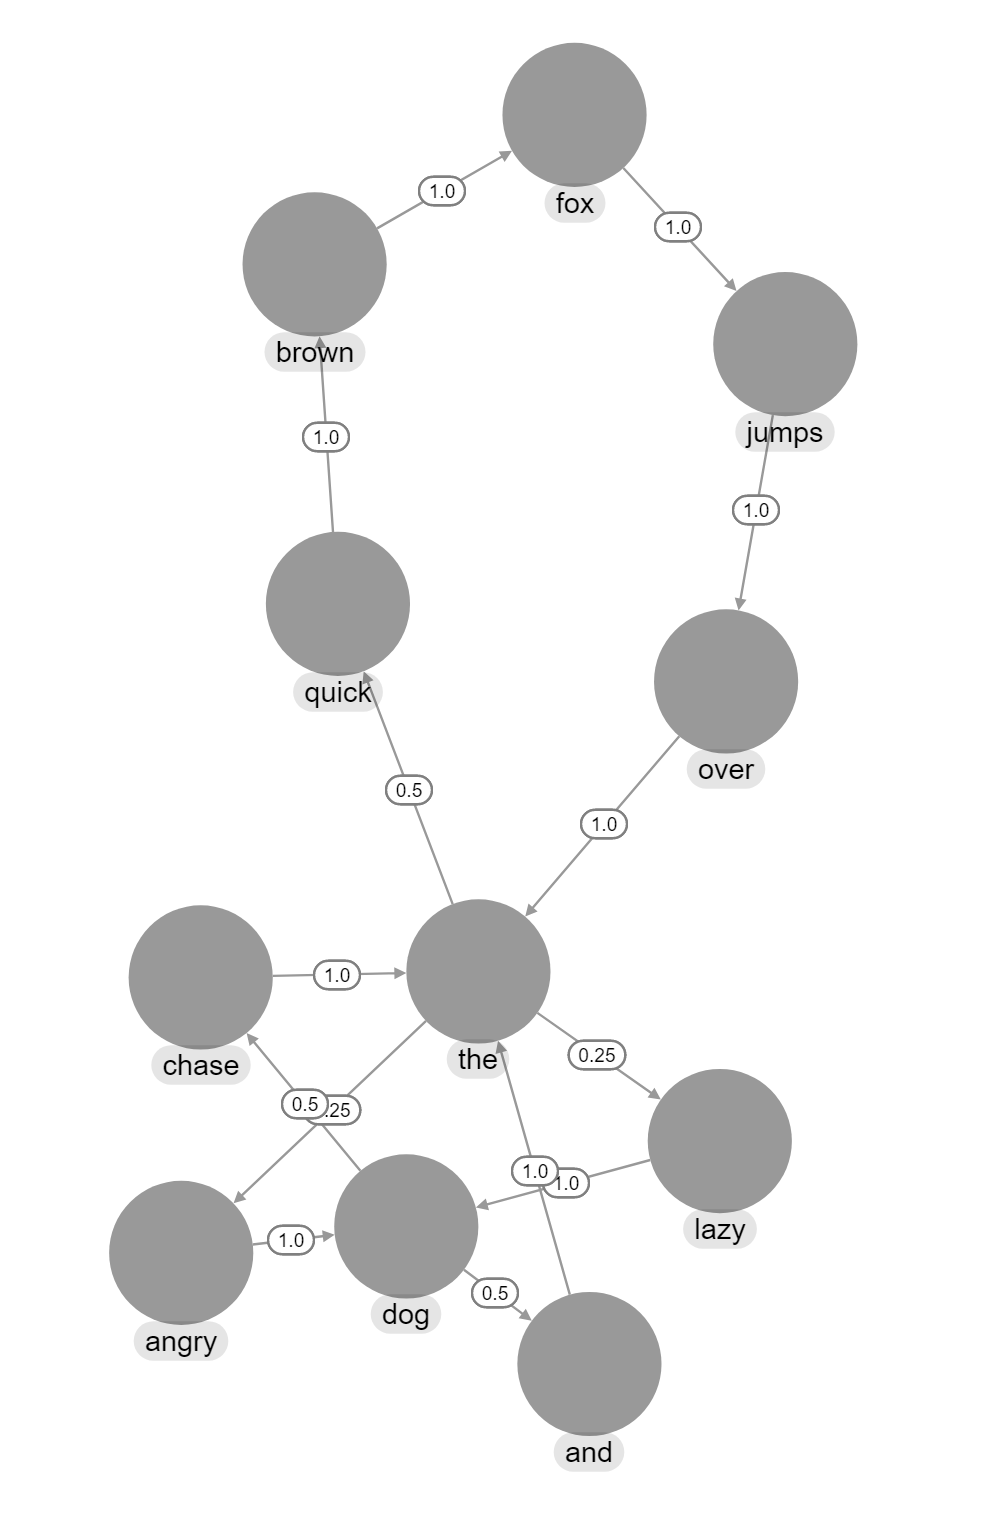
\includegraphics[width=0.75\textwidth]{chain}
    \caption{Przykład łańcucha Markova, dla zdania "The quick brown fox jumps over the lazy dog and the angry dog chase the quick brown fox.", dla wartości $ngram = 1$, oznaczającej stany jako pojedyncze słowama oraz wartoścami prawdopodobieństw przejść pomiędzy stanami obliczonych na podstawie zdania wejściowego.}
    \label{fig:mesh1}
\end{figure}
\FloatBarrier
\subsection{Prawo Zipfa}
Prawo Zipfa to empiryczna obserwacja dotycząca częstotliwości występowania słów w korpusie tekstów. Mówi ono, że jeśli posortujemy słowa występujące w tekście według częstotliwości ich wystąpień i przyporządkujemy każdemu słowu rangę zgodną z jego pozycją w rankingu, to liczba wystąpień słowa o danej randze jest odwrotnie proporcjonalna do wartości tej rangi. W praktyce oznacza to, że najczęściej występujące słowo będzie występować dwa razy częściej niż drugie na liście, trzy razy częściej niż trzecie, i tak dalej. \\
\\
Wykorzystując Prawo Zipfa w generacji tekstów piosenek, można zapewnić, że wygenerowany tekst będzie przypominał rzeczywiste teksty pod względem częstotliwości występowania słów.
\begin{figure}
     \centering
     \begin{subfigure}[b]{0.75\textwidth}
         \centering
         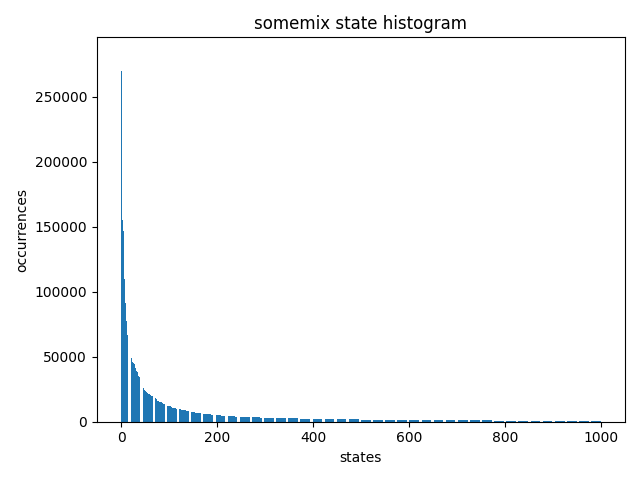
\includegraphics[width=\textwidth]{somemix_zipf1}
         \caption{Wykres 1000 najczęściej pojawiających się słów dla zbioru danych $somemix.csv$.}
         \label{fig:mesh1}
     \end{subfigure}
     \hfill
     \begin{subfigure}[b]{0.75\textwidth}
         \centering
         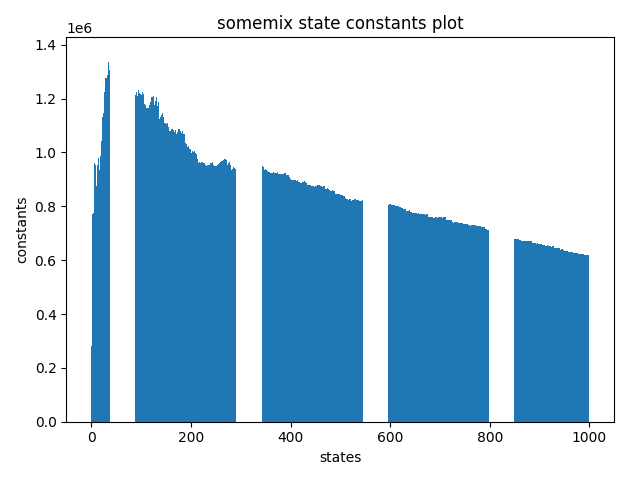
\includegraphics[width=\textwidth]{somemix_zipf2}
         \caption{Wykres stałej $constant = ranga * wystapienia$ dla zbioru danych $somemix.csv$}
         \label{fig:mesh1}
     \end{subfigure}
\end{figure}
\FloatBarrier
\begin{figure}
     \centering
     \begin{subfigure}[b]{0.75\textwidth}
         \centering
         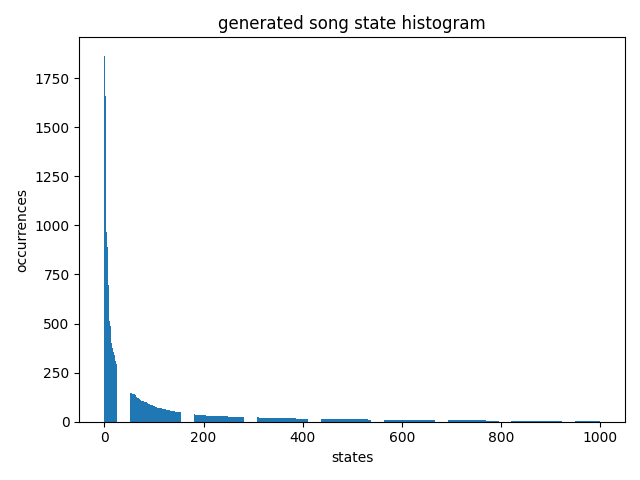
\includegraphics[width=\textwidth]{generated_zipf1}
         \caption{Wykres 1000 najczęściej pojawiających się słów dla piosenki wygenerowanej na podstawie $somemix.csv$ o 100 wersach po 500 słów.}
         \label{fig:mesh1}
     \end{subfigure}
     \hfill
     \begin{subfigure}[b]{0.75\textwidth}
         \centering
         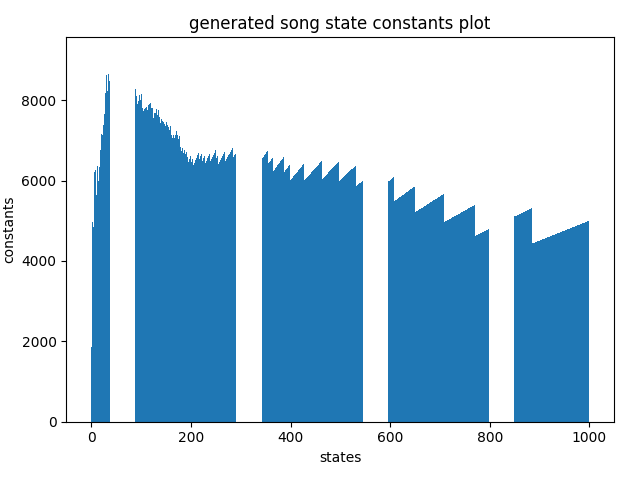
\includegraphics[width=\textwidth]{generated_zipf2}
         \caption{Wykres stałej $constant = ranga * wystapienia$  dla piosenki wygenerowanej na podstawie $somemix.csv$ o 100 wersach po 500 słów}
         \label{fig:mesh1}
     \end{subfigure}
\end{figure}
\FloatBarrier
Podobieństwo wykresów wskazuje na to, że tekst wyjściowy modelu będzie tej samej jakości, przypominając tekst dany na wejściu.
\subsection{Prawo Heapsa}
Prawo Heapsa opisuje zależność pomiędzy wielkością dokumentu w jednostce liter, słów, stanów złożonych ze słów w kontekście liczby unikalnych liter, słów, stanów złożonych ze słów pojawiających się w tekście. Na podstawie prawa, stwierdzamy, że liczba unikalnych stanów rośnie wolniej wraz ze zwiększającą się ilością stanów tekstu, co pozwala nam przewidzieć ilość unikalnych w zasobie danych, co pozwala na lepszą ocenę modelu Markova.
\begin{figure}
     \centering
     \begin{subfigure}[b]{0.49\textwidth}
         \centering
         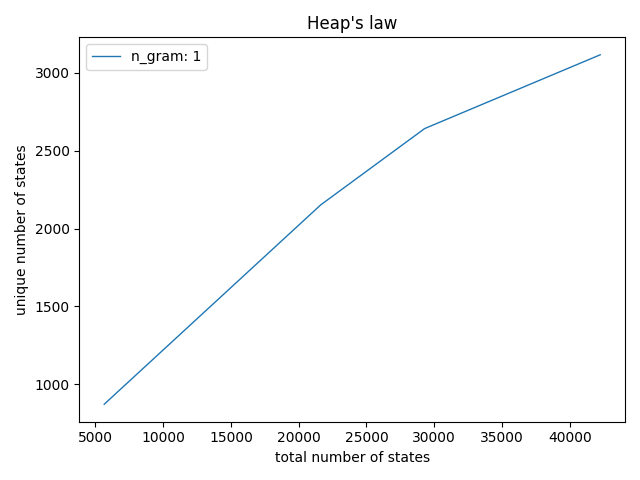
\includegraphics[width=\textwidth]{heaps1}
         \label{fig:mesh1}
     \end{subfigure}
     \hfill
     \begin{subfigure}[b]{0.49\textwidth}
         \centering
         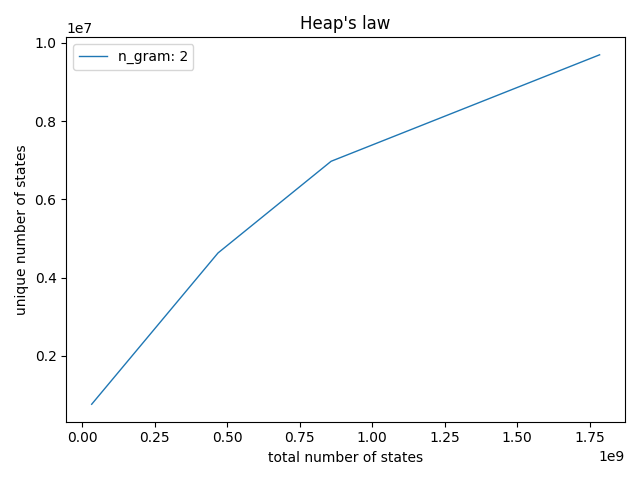
\includegraphics[width=\textwidth]{heaps2}
         \label{fig:mesh1}
     \end{subfigure}
     \hfill
     \begin{subfigure}[b]{0.49\textwidth}
         \centering
         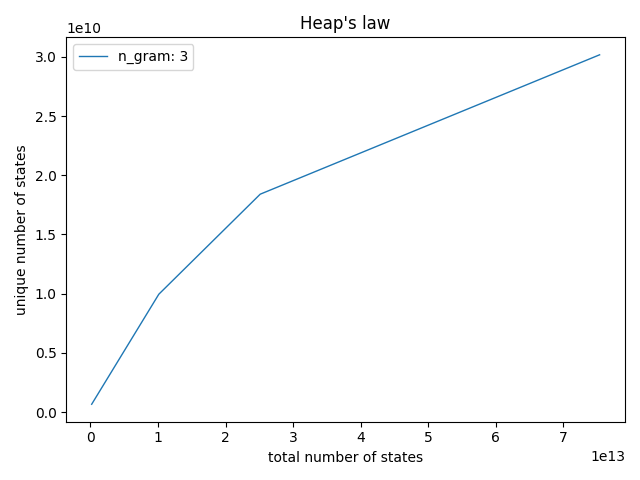
\includegraphics[width=\textwidth]{heaps3}
         \label{fig:mesh1}
     \end{subfigure}
     \hfill
     \begin{subfigure}[b]{0.49\textwidth}
         \centering
         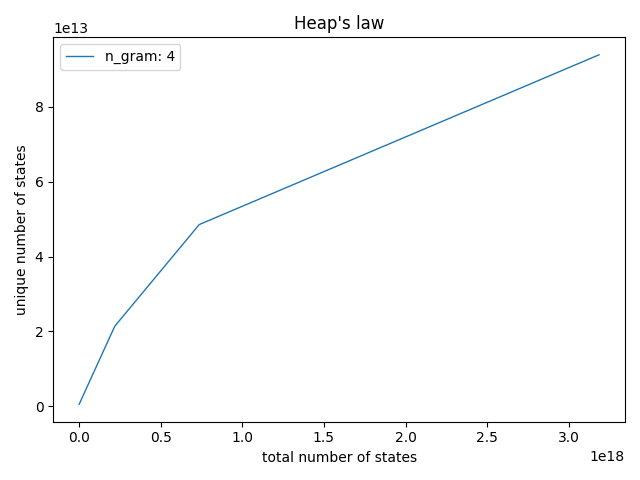
\includegraphics[width=\textwidth]{heaps4}
         \label{fig:mesh1}
     \end{subfigure}
     \hfill
     \begin{subfigure}[b]{0.49\textwidth}
         \centering
         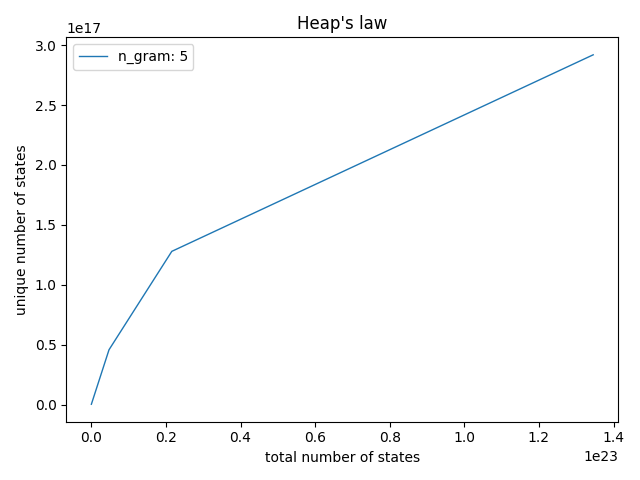
\includegraphics[width=\textwidth]{heaps5}
         \label{fig:mesh1}
     \end{subfigure}
     \hfill
        \caption{Wykres zależności liczby stanów unikalnych od rozmiaru tekstu oraz wartości $ngram$ dla zbiorów danych: $kyuss.csv, led\_zeppelin.csv, Black Sabbath.csv, ac\_dc.csv$.}
        \label{fig:mesh1}
\end{figure}
\FloatBarrier
Prawo Heapsa sprawdza się dla danych. Dodatkowo widzimy, że zmiana jest zależna od $ngramu$. Rośnie ona zwykle wolniej dla większych $ngramow$ co może oznaczać częste pojawianie się w tekstach określonych złożeń słów.
\subsection{Entropia Krzyżowa}
Entropia Krzyżowa to miara zgodności między dwoma rozkładami prawdopodobieństwa. Pozwala określić jak dobrze model generujący tekst przewiduje następny stan na podstawie poprzednich. W przypadku generowania tekstu, entropia krzyżowa może być wykorzystana do oceny jakości generacji. Im mniejsza wartość entropii krzyżowej, tym większa zgodność między rozkładem prawdopodobieństwa generowanego tekstu a rozkładem prawdopodobieństwa prawdziwych tekstów. Pozwala to ocenić czy model tworzy teksty podobne do tych ze zbioru danych, czy też tworzy nowe i oryginalne sentencje.
\\\\
Obliczanie Entropii krzyżowej:
\begin{itemize}
    \item Tworzymy rozkład prawdopodobieństwa wygenerowanego tekstu, zależnie od używanych n-gramów.
    \item Iterując po każdym n-gramie tekstu wygenerowanego obliczamy sumę iloczynów logarytmu prawdopodobieństwa wystąpienia następnego słowa w modelu oraz prawdopodobieństwa wystąpienia następnego słowa w rozkładzie wygenerowanego tekstu. \\\\ $-\sum log(P(M)) * P(L)$ \\ , gdzie $P(M)$ oznacza prawdopodobieństwa wystąpienia następnego słowa w modelu, a $P(L)$ prawdopodobieństwa wystąpienia następnego słowa w rozkładzie wygenerowanego tekstu.
\end{itemize}
\begin{figure}[h]
    \centering
    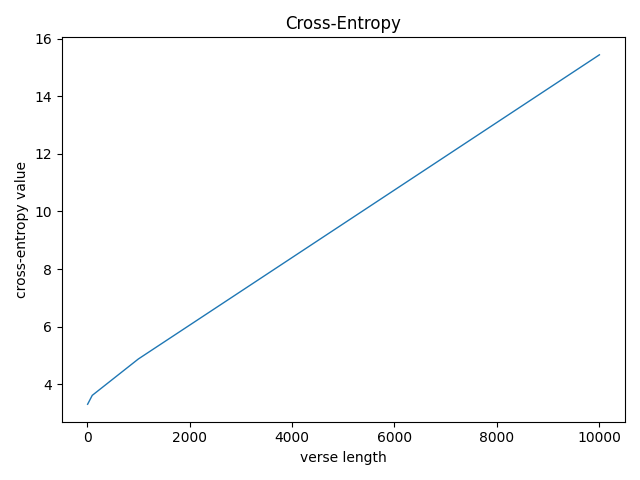
\includegraphics[width=0.75\textwidth]{cross-entropy}
    \caption{Wykres wartości entropii krzyżowej dla tekstu generowanego na podstawie zbioru danych $somemix.csv$, zależnie od rozmiaru wygenerowanego tekstu.}
    \label{fig:mesh1}
\end{figure}
\FloatBarrier
Jak widać, entropia krzyżowa rośnie niemal liniowo względem długości wygenerowanego tekstu. Oznacza to, że model coraz to bardziej generuje tekst niepodobny do oryginalnego zależnie od długości wygenerowanego tekstu.
\subsection{Perpleksja}
Perpleksja to stopień trudności zrozumienia tekstu, miara nieprzewidywalności modelu. Im niższa tym tekst bardziej przypomina oryginalny i jest bardziej kreatywny. Aby policzyć wartość perpleksji tekstu korzystamy ze wzoru: $Perplexity(M) = 2^{H(L,M)}$ gdzie $M$ oznacza model, $L$ oznacza wygenerowany tekst, a $H(L, M)$ wartość entropii krzyżowej.
\begin{figure}[h]
    \centering
    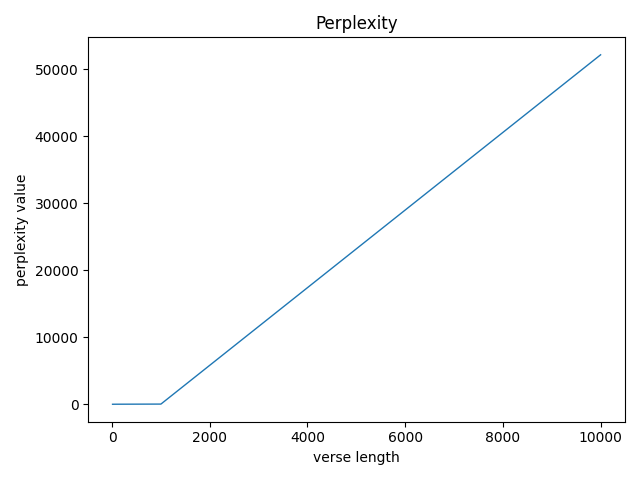
\includegraphics[width=0.75\textwidth]{perplexity}
    \caption{Wykres wartości perpleksji dla tekstu generowanego na podstawie zbioru danych $somemix.csv$, zależnie od rozmiaru wygenerowanego tekstu.}
    \label{fig:mesh1}
\end{figure}
\FloatBarrier
Jak widać, wykresy eksperymentu dla entropii krzyżowej i perpleksji się nie różnią, ponieważ w gruncie rzeczy znaczą tą samą miarę.
\subsection{Self-BLEU}
Self-BLEU określa różnorodność generowanego tekstu. Wykorzystuje wskaźnik \href{https://pl.wikipedia.org/wiki/BLEU}{BLEU} (ang. BiLingual Evaluation Understudy), licząc jego wartość dla kombinacji par wszystkich unikalnych sentencji wygenerowanego tekstu, w tym przypadku wersów piosenki, otrzymując końcowo ich średnią. Im mniejsza wartość wskaźnika tym większa różnorodność w tekście. Metryka pozwala uniknąć monotonności tekstu. \\\\
Sam wskaźnik BLEU mierzy podobieństwo między tłumaczeniem maszynowym a jednym lub wieloma tłumaczeniami referencyjnymi poprzez porównanie stopnia pokrycia n-gramów (ciągów po n kolejnych słów) między nimi. Im wyższy wynik, tym większe podobieństwo między tłumaczeniem a referencją. Wartości wskaźnika BLEU mieszczą się w przedziale od 0 do 1, gdzie 1 oznacza idealne dopasowanie tłumaczenia maszynowego do referencji. W praktyce, oczekuje się wyników BLEU powyżej 0,4-0,5, aby uznać tłumaczenie maszynowe za akceptowalne.\\
\begin{figure}[h]
    \centering
    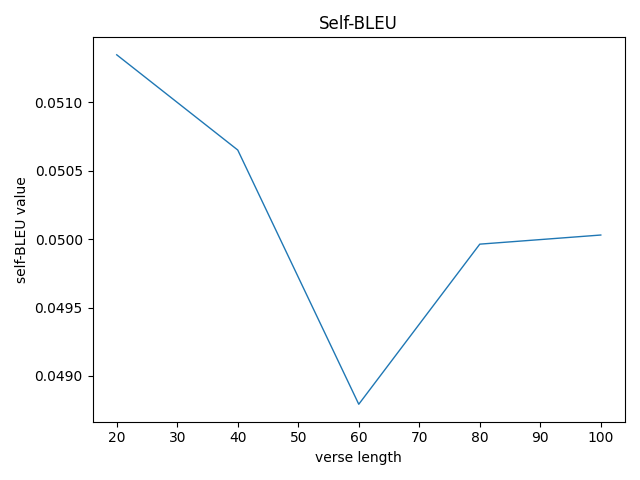
\includegraphics[width=0.75\textwidth]{self-bleu}
    \caption{Wykres wartości Self-BLEU dla tekstu generowanego na podstawie zbioru danych $somemix.csv$, zależnie od rozmiaru wygenerowanego tekstu.}
    \label{fig:mesh1}
\end{figure}
\FloatBarrier
Jak widać, tekst zachowuje wysoką różnorodność, poprzez losowy wybór początku wersu rozkładem równomiernym, a z coraz to większym rozmiarem tekstu napotykamy na nowe frazy, co zwiększa jego różnorodność, jednak wciąż wynik jest zależny od wygenerowanych tekstów.
\FloatBarrier
\subsection{Przykładowe wyniki}
\newpage
\begin{center}
    Przykładowe wyniki generacji 10 wersów po 10 słów dla zbioru danych $english\_mixtape.csv$: \\
    \leavevmode\\
    \textsl{Shy yeah repeat everything i want you hard dont get \\
            Slow with plenty of desperation in the night end of \\
            Until that day lost my way you bat your eyes \\
            Back baby cause your man is back wonder where you \\
            Under water forever was their faith i will let you \\
            Windows feel like giving up cause you know theres only \\
            Lets shout lets make it baby now worry like lying \\
            Some room for you and me can you heal what \\
            Shot cmon terminator uzi makers regulators gon na blow my \\
            A poto over the road youre on your move what} \\
    \leavevmode\\\leavevmode\\
    Przykładowe wyniki generacji 10 wersów po 10 słów dla zbioru danych $somemix.csv$: \\
    \leavevmode\\
    \textsl{Hell forget about me making a movie turn on a \\
            Bas en haut jaimais manger sa peau je sais que \\
            Main banu tera ehsaas main yaar banavanga akhiyaan milavanga akhiyaan \\
            So stroke me and no reason to believe that parted \\
            Now sexy dance sexy dancer hot as hades early eighties \\
            How sophisticated you know what they do they laugh and \\
            Of brotherly love the feel of silk and your talents \\
            Goddamn alotta brilliant bitch have it you be not much \\
            Line trill tell me youre always gon na need your \\
            Crawling on them haters sick itd be worth more dan} \\
    \leavevmode\\\leavevmode\\
\end{center}
\newpage
\section{Rekurencyjne Sieci Neuronowe}
    \subsection{Wstęp o rekurencyjnych sieciach neuronowych}
    Rekurencyjne sieci neuronowe (RNN) są specjalnym rodzajem sieci neuronowych, które mają zdolność do uwzględniania kontekstu sekwencji danych. Oznacza to, że RNN są w stanie analizować dane wejściowe w sposób sekwencyjny, zachowując informacje o poprzednich krokach. Ta cecha czyni je szczególnie skutecznymi w modelowaniu danych sekwencyjnych, takich jak język naturalny, dźwięk czy szereg czasowy.\\\\
Podstawowym elementem rekurencyjnej sieci neuronowej jest rekurencyjna jednostka, która wykonuje operację na aktualnym kroku czasowym oraz przechowuje stan, który jest przekazywany do następnego kroku. Najpopularniejszym typem jednostki rekurencyjnej jest jednostka LSTM (Long Short-Term Memory) oraz GRU (Gated Recurrent Unit). Obie te jednostki są zaprojektowane w taki sposób, aby rozwiązywać problem znikającego i eksplodującego gradientu, który często występuje podczas uczenia rekurencyjnych sieci neuronowych.\\\\
W trakcie uczenia rekurencyjnej sieci neuronowej wsteczna propagacja błędu jest stosowana w celu minimalizacji błędu wyjścia. Jednak w odróżnieniu od tradycyjnych sieci jednokierunkowych, RNN używają również propagacji wstecznej w czasie, aby rozprowadzić gradienty przez wszystkie kroki czasowe. Dzięki temu sieć jest w stanie uczyć się na podstawie kontekstu historycznego i uwzględniać informacje z poprzednich kroków.\\\\
Rekurencyjne sieci neuronowe jednak nie są pozbawione wad. Jednym z problemów jest trudność w uczeniu długotrwałych zależności, ponieważ gradienty mogą zanikać lub eksplodować w czasie. W praktyce często stosuje się różne techniki, takie jak LSTM czy GRU, aby radzić sobie z tym problemem. Ponadto, obliczenia w rekurencyjnych sieciach neuronowych są bardziej czasochłonne niż w przypadku sieci jednokierunkowych, co może stanowić wyzwanie w przypadku dużych zbiorów danych.\\\\
Podsumowując, rekurencyjne sieci neuronowe są potężnym narzędziem do analizy danych sekwencyjnych. Dzięki swojej zdolności do uwzględniania kontekstu historycznego, są one szczególnie skuteczne w modelowaniu danych sekwencyjnych. Jednak ich skomplikowana natura i trudności w uczeniu długotrwałych zależności wymagają starannego projektowania i optymalizacji.
    \begin{figure}[h]
        \centering
        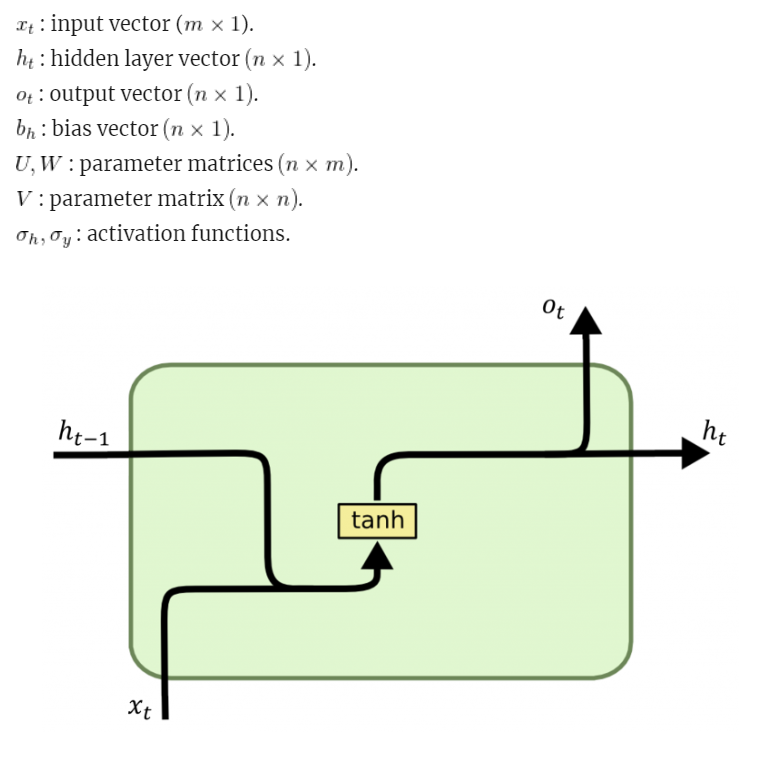
\includegraphics[width=0.75\textwidth]{images/rnn.png}
        \caption{Obrazek przedstawia schemat działania Recurrent Neural Network.}
        \label{fig:mesh1}
    \end{figure}
    \pagebreak
    \subsection{LSTM}
    LSTM (Long Short-Term Memory) to rodzaj rekurencyjnej jednostki używanej w rekurencyjnych sieciach neuronowych (RNN), która rozwiązuje problem znikającego gradientu. Składa się z bramek wejściowej, zapominającej i wyjściowej, które kontrolują przepływ informacji. Jednostka LSTM ma zdolność do przechowywania informacji przez wiele kroków czasowych dzięki mechanizmowi "ścieżki pamięci"
    \begin{figure}[h]
        \centering
        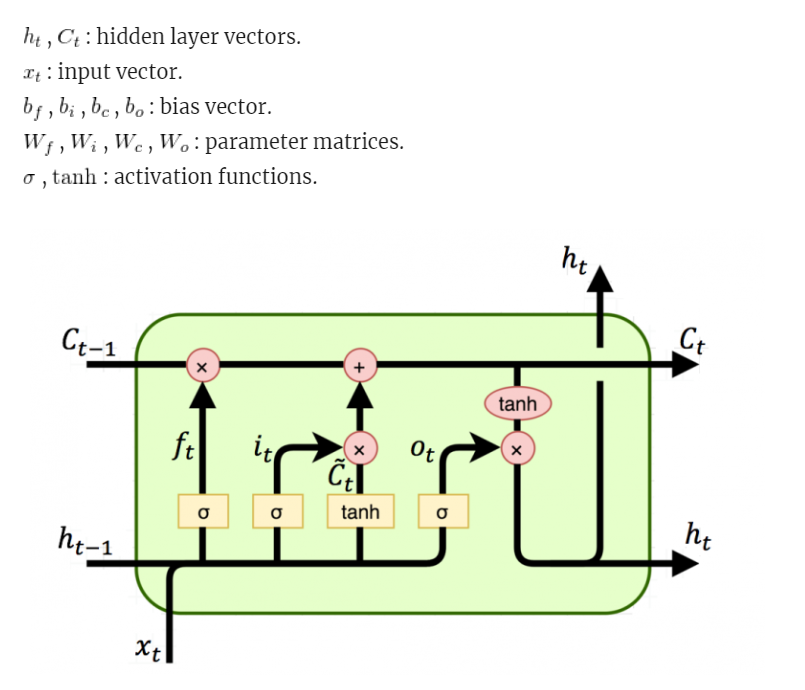
\includegraphics[width=0.75\textwidth]{images/lstm.png}
        \caption{Obrazek przedstawia schemat działania Long-Short Term Memory.}
        \label{fig:mesh1}
    \end{figure}
    \pagebreak
    \subsection{GRU}
    GRU (Gated Recurrent Unit) to rodzaj jednostki w rekurencyjnych sieciach neuronowych (RNN), której struktura obejmuje bramki resetowania i aktualizacji. Działa podobnie do LSTM, umożliwiając skuteczne modelowanie długotrwałych zależności w danych sekwencyjnych. GRU ma mniejszą liczbę parametrów niż LSTM, a mimo to osiąga podobne efektywności. Jest popularnym rozwiązaniem w przetwarzaniu języka naturalnego, rozpoznawaniu mowy i generowaniu tekstu.
    \begin{figure}[h]
        \centering
        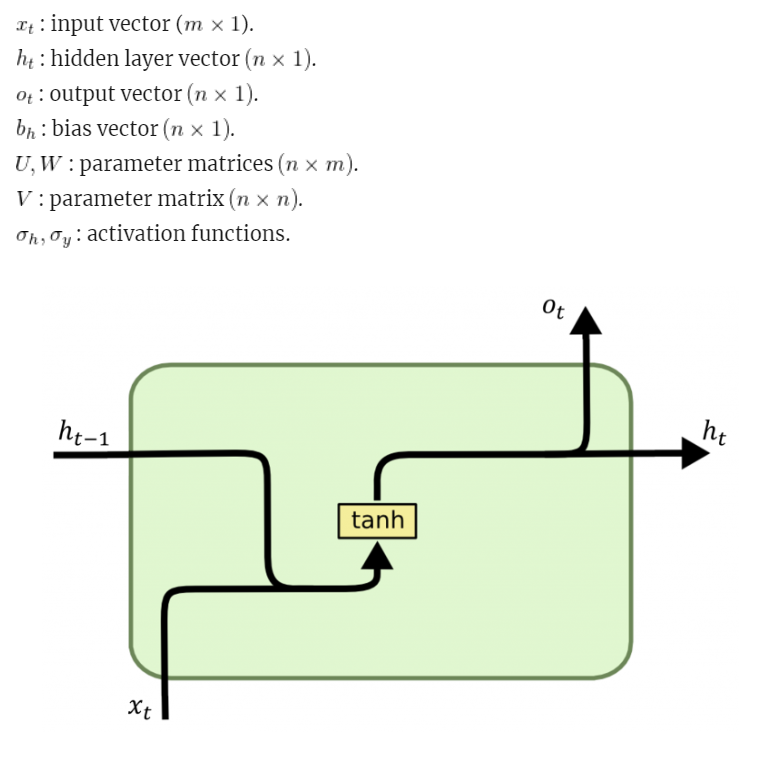
\includegraphics[width=0.75\textwidth]{images/rnn.png}
        \caption{Obrazek przedstawia schemat działania Gated Recurrent Unit.}
        \label{fig:mesh1}
    \end{figure}
    \pagebreak
    \subsection{Różnice między LSTM, a GRU}
    GRU i LSTM są dwoma popularnymi typami jednostek w rekurencyjnych sieciach neuronowych (RNN). GRU ma prostszą strukturę, mniejszą liczbę parametrów i bramki resetowania. LSTM ma bardziej złożoną strukturę, oddzielną komórkę pamięci i trzy bramki. Wybór między nimi zależy od kontekstu i danych sekwencyjnych.
    \subsection{Problem znikającego gradientu}
    Problem znikającego gradientu występuje w rekurencyjnych sieciach neuronowych (RNN), gdy gradienty maleją wraz z propagacją wsteczną przez kolejne kroki czasowe. To utrudnia naukę długotrwałych zależności. Jednostki LSTM i GRU zostały opracowane w celu rozwiązania tego problemu, umożliwiając skuteczniejsze modelowanie długoterminowych zależności w danych sekwencyjnych.
    \subsection{Embedding}
    Embedding w rekurencyjnych sieciach neuronowych (RNN) to proces przekształcania dyskretnych elementów, takich jak słowa lub symbole, na gęste wektory o niskiej wymiarowości. W przypadku analizy języka naturalnego, embeddingi są używane do reprezentowania słów lub sekwencji słów w sposób, który zachowuje ich semantykę i relacje między nimi.\\\\
Podstawowym celem embedingu w RNN jest przechwycenie znaczenia słów lub sekwencji słów w sposób, który umożliwia modelowi RNN efektywne przetwarzanie i wnioskowanie na podstawie tych danych. Embeddingi są trenowane wraz z resztą sieci RNN i są aktualizowane podczas procesu uczenia. \\\\
Proces embedingu zaczyna poprzez przypisania do unikalnego wektora liczba rzeczywistych dla każdego słowa, losowych wartości. Będą one aktualizowane podczas uczenia, aby zwiększyć strukturę symetralną języka. Istotną kwestią jest aby słowa o podobnym znaczeniu miały bliskie sobie wektory, dzięki czemu model RNN może wykrywać podobieństwa i zależności między słowami w trakcie analizy tekstu.

\newpage
\section{Sieci neuronowe na transformatorach}
\subsection{Przykładowe wykorzystanie sieci neuronowych na transformatoarach:}
    \begin{itemize}
        \item przewidywania kolejnego słowa
        \item tłumaczenia z innego języka
        \item odpowiadania na pytania
        \item podsumowywania dokumentu
        \item parafrazowania
        \item tworzenia nowego tekstu
        \item gry w szachy
        i wielu innych 
    \end{itemize}
Modele językowe takie jak BERT, GPT-2 czy GPT-3 wykorzystują właśnie transformatory. Ale przyjżyjmy się jak działa transformator?
\subsection{Analiza działania transformera:}
    \begin{figure}[h]
        \centering
        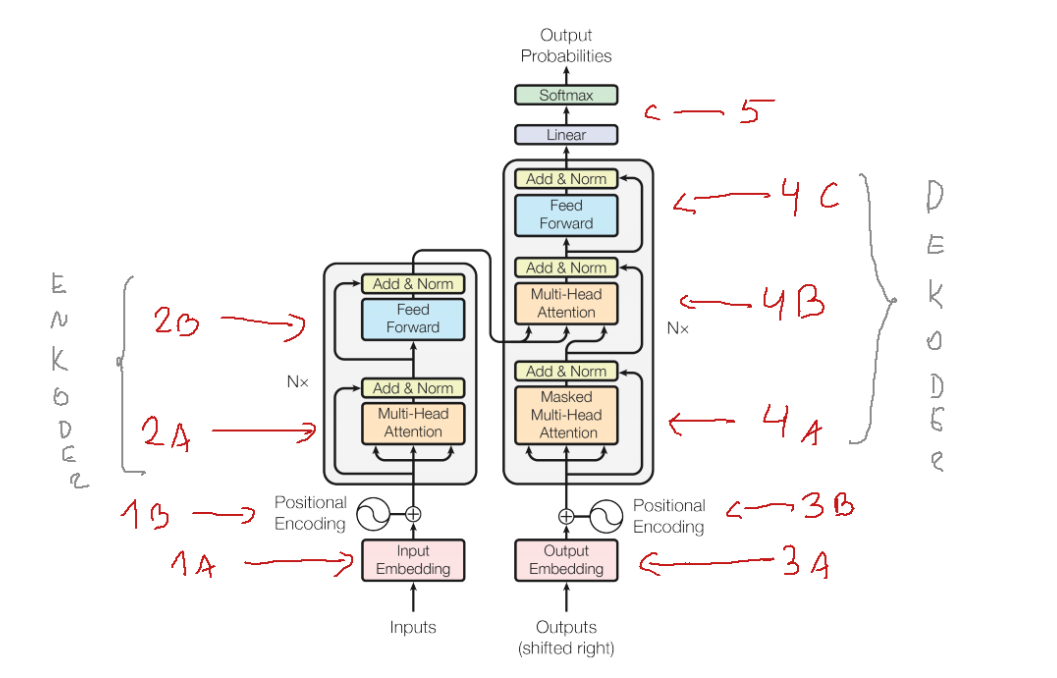
\includegraphics[width=0.75\textwidth]{images/Schemat-dzialania.png}
        \caption{Obrazek przedstawia schemat działania tranformera z opisami potrzebnymi do dalszego opisu.}
        \label{fig:mesh1}
    \end{figure}
    \begin{description}
      \item[1A] \hfill \\
      Embedding (osadzenie) to proces zamiany słów na liczby lub wektory, które można przetwarzać za pomocą modelu. Słowa są mapowane na przestrzeń wielowymiarową, gdzie podobne słowa są blisko siebie, a różne słowa są oddalone od siebie. Embedding jest podstawowym krokiem w procesie przetwarzania tekstu w modelach językowych.
      \item[1B ] \hfill \\
      Positional encoding (kodowanie pozycyjne) to technika, która dodaje informację o pozycji słowa do jego osadzenia (embedding). Pozwala to modelowi uwzględnić kontekst i kolejność słów w zdaniu. Wektory kodowania pozycji są dodawane do wektorów embeddingowych, aby utworzyć reprezentację wektorową słowa z uwzględnieniem kontekstu.
      \item[2A ] \hfill \\
      Multi-head attention to mechanizm, który pozwala modelowi na skupienie się na różnych częściach zdania jednocześnie. Jest obliczany dla każdego słowa i bierze pod uwagę zarówno samo słowo, jak i kontekst między słowami. W efekcie otrzymujemy wektor uwagi dla każdego słowa.
      \begin{figure}[h]
        \centering
        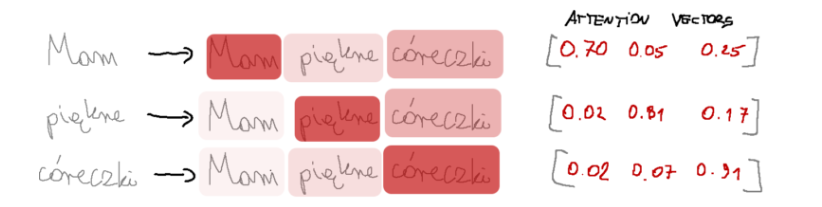
\includegraphics[width=0.75\textwidth]{images/wektor-uwagi.png}
        \caption{Obrazek przedstawia schemat działania wekotra uwagi.}
        \label{fig:mesh1}
    \end{figure}
      \item[2B  ] \hfill \\
      Feed-forward network (sieć jednokierunkowa) to warstwa w transformerze, która przekształca wektory uwagi dla każdego słowa. Każdy wektor jest przekazywany przez sieć wielowarstwową, która działa niezależnie dla każdego słowa. Ten proces można zrównoleglić, co przyspiesza obliczenia.
      \begin{figure}[h]
        \centering
        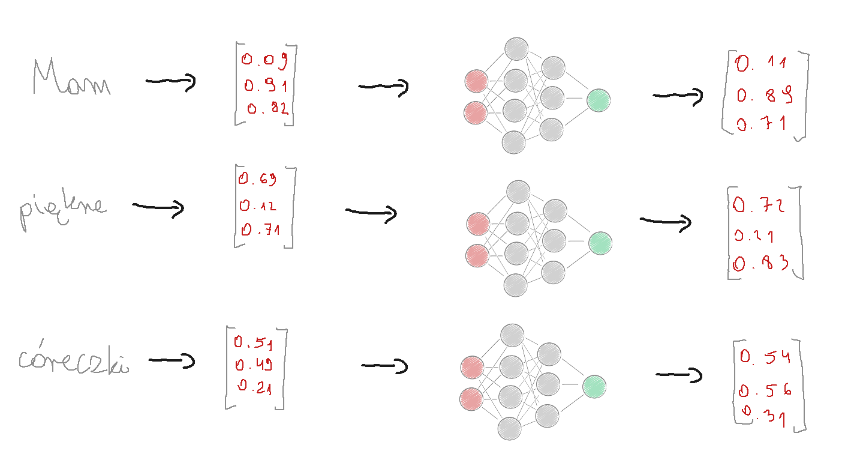
\includegraphics[width=0.75\textwidth]{images/siec-wielowarstowa.png}
        \caption{Obrazek przedstawia schemat działania wekotra uwagi.}
        \label{fig:mesh1}
    \end{figure}
      \item[3A i 3B ] \hfill \\
      W tych krokach powtarza się proces opisany w 1A i 1B. Dane wejściowe to wynikowe zdanie, a wynikiem jest zaktualizowana reprezentacja wektorowa zdania z uwzględnieniem kontekstu i pozycji słów.
      \item[4A  ] \hfill \\
      Masked multi-head attention (uwaga wielogłowicowa z maskowaniem) jest wykorzystywana w dekoderze modelu transformerowego. Maskowanie pozwala na przetwarzanie sekwencji w sposób sekwencyjny, bez łamania kierunku czasowego. Modele transformers z maskowaniem mogą generować predykcje sekwencyjne, nie mając informacji o przyszłych elementach sekwencji.
      \begin{figure}[h]
        \centering
        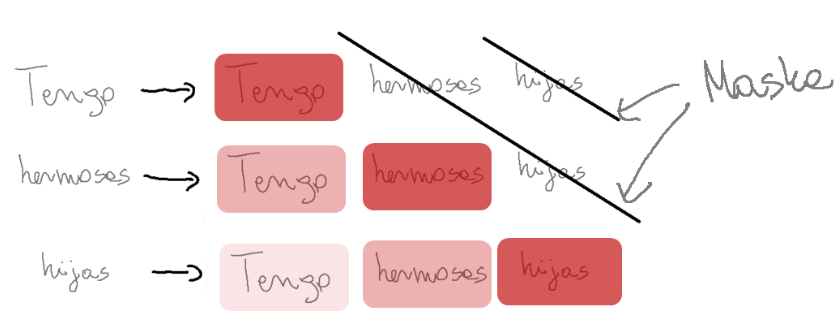
\includegraphics[width=0.75\textwidth]{images/maska.png}
        \caption{Obrazek przedstawia schemat działania maskowania na przykładzie zdania po języku hiszpańskim, które ma być przetłumaczone na inny język.}
        \label{fig:mesh1}
    \end{figure}
      \item[4B ] \hfill \\
      Multi-head attention w dekoderze to proces porównywania wektorów uwagi między dekoderem a enkoderem. Sprawdza on jakość powiązania między wektorami słów w obu częściach modelu, aby model mógł zrozumieć, jak różne słowa są ze sobą powiązane.
      \item[4C  ] \hfill \\
      Feed-forward network jest ponownie stosowane w dekoderze w celu uproszczenia wektorów uwagi i ułatwienia dalszego przetwarzania przez model.
      \item[5 ] \hfill \\
      Na końcu wynik z transformera przekazywany jest przez warstwę liniową (linear layer), która przekształca wyniki w wymiarze odpowiadającym liczbie słów w zdaniu. Następnie funkcja softmax zamienia wyniki w prawdopodobieństwa, które można interpretować jako pewność modelu co do przynależności słów do różnych kategorii lub etykiet.
    \end{description}
\subsection{Wady i zalety:}
    \begin{description}
      \item[Zalety] \hfill \\
      Główną zaletą transformerów jest szybkość działania w porównaniu z siecią RNN lub LSTM. Ponadto elementem, który wpływa na to, że coraz chętniej się po nie sięga, są dużo lepsze wyniki w porównaniu z innymi algorytmami.
      \item[Wady] \hfill \\      
        \begin{itemize}
          \item potrzeba dużej mocy obliczeniowej, aby zostały wytrenowane
          \item potrzeba naprawdę dużej ilości danych do wytrenowania
          \item dostępne są przykłady, że gorzej sobie radzą z hierarchicznymi danymi
          \item w związku z tym, że są stosunkowo nowe, to w przypadku błędów możliwe, że informacja o jego naprawieniu będzie ciężka do znalezienia w internecie.
        \end{itemize}
    \end{description}
\newpage
\section{GPT-2}
GPT-2 (Generative Pre-trained Transformer 2) to zaawansowany model językowy oparty na architekturze transformer. Został opracowany przez OpenAI i jest jednym z najbardziej znanych i potężnych modeli generatywnych opartych na uczeniu maszynowym.\\\\
GPT-2 ma zdolność do generowania wysokiej jakości tekstu, co sprawia, że jest bardzo przydatny w różnych zastosowaniach, takich jak generowanie treści, redagowanie, tłumaczenie i wiele innych. Model ten został wytrenowany na ogromnych zbiorach danych tekstowych z internetu, co pozwoliło mu na zdobycie ogromnej wiedzy na temat języka naturalnego.\\\\
Jednym z kluczowych elementów GPT-2 jest jego zdolność do kontekstowego rozumienia tekstu. Dzięki warstwom transformer i mechanizmowi uwagi, model jest w stanie analizować kontekst i zależności między słowami, co prowadzi do generowania bardziej spójnych i sensownych tekstów.\\\\
GPT-2 wykorzystuje uczenie nienadzorowane, co oznacza, że jest trenowany na dużych zbiorach danych bez konkretnych etykiet czy celów zadania. Wytrenowany model jest w stanie generować teksty na podstawie danego kontekstu, a jakość generacji zależy od jakości danych treningowych i rozmiaru modelu.\\\\
Warto zaznaczyć, że GPT-2 ma również pewne ograniczenia. Ze względu na to, że jest oparty na uczeniu maszynowym nienadzorowanym, może generować nieodpowiednie, niepoprawne lub niezgodne z rzeczywistością treści, co dla niektórych niestety może być zaletą. Ponadto, model może być podatny na wprowadzanie błędnych informacji, które znalazły się w danych treningowych.\\\\
\textbf{Jako generator obrazów}\\\\
W tym momencie GPT jest wykorzystywany również jako generator obrazów. Nieco ponad miesiąc po premierze GPT-3, superpotężnego algorytmu generującego tekst, jego poprzednik – GPT-2 – znalazł nowe wcielenie. Jego twórcy postanowili sprawdzić, jak ich model zachowałby się, gdyby wyszkolić go nie na terabajtach tekstu, ale na milionach fotografii.\\\\
Otóż modele typu Transformer, do których należy GPT-2, określa się jako domain-agnostic, czyli niezależne od przetwarzanych danych. Oznacza to, że model teoretycznie zadziała dla każdych danych, które można zamienić na jednowymiarową sekwencję.\\\\
Tekst jest taką sekwencją z natury, ale co z dwuwymiarowym obrazem? Żeby to zadziałało, trzeba go było rozłożyć na czynniki pierwsze – obraz został „linijka po linijce” zapisany jako ciąg pikseli. Każdy piksel z osobna został zakodowany w specjalnie zaprojektowanym dziewięciobitowym systemie określania koloru.\\\\
Okazało się, że algorytm działający na jednowymiarowych sekwencjach danych, którego działanie w wielkim uproszczeniu sprowadza się do przewidywania kolejnego elementu układanki z zachowaniem kontekstu całości, świetnie sprawdza się także w generowaniu dwuwymiarowych obrazów.\\\\
Jeśli dać mu fragmet obrazu to wytworzy spójny stylistycznie ciąg dalszy i to w różnych wariantach. To nie ma na celu odtworzenie orginału, ale coś nowego o różnych wariantach. Efekt jest analogiczny jak w przypadku generowania tekstu – dalszy ciąg jest całkowicie zmyślony, ale stylistycznie spójny z początkowym fragmentem. Próbki działania algorytmu można zobaczyć na poniższej ilustracji.
\begin{figure}[h]
        \centering
        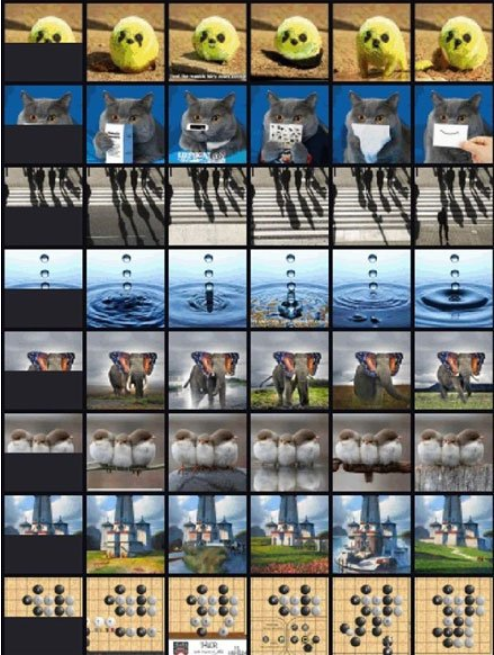
\includegraphics[width=0.75\textwidth]{images/obrazki.png}
        \caption{Obrazek przedstawia schemat działania gpt-2 na obrazach.}
        \label{fig:mesh1}
    \end{figure}
\end{document}
